\section{Results and discussion}
\subsection{$NVT$ simulation - build-up of interfacial charge}
The interaction between the toluene film and the surrounding water molecules and ions results in a dynamic charge distribution. The Figure \ref{fig:nvt_charges_all_voltage} illustrates the ion (sodium and chlorine) charge density  distribution in the $z$-direction. The distribution is computed within the last $2.5\, ns$ of the run (total run time $5\, ns$).  The three curves correspond to  $0$, $60$ and $100\, mV/nm$ strengths of the external electric field. At $0\, mV/nm$ (red curve), which calibrates the results, the charge  fluctuates around zero at the film interfaces. A non-zero external field induces charge accumulation at film interfaces. The accumulated charge is drawn as peaks in the charge distribution. The curves for  $60\, mV/nm$  (green) and $100\, mV/nm$ (blue) electric field strengths show that the accumulated charge increases with the  field increase: one interface of the toluene film is charged positively due to $Na^+$ accumulation, while the other interface  is charged negatively due to  $Cl^-$ ion accumulation.  Thus, the emulsion film, subjugated to the external electric field, resembles charging of a parallel-plate capacitor. At all applied fields the ion charge fluctuates around zero away from the film. 


\begin{figure}[ht]
\begin{center}
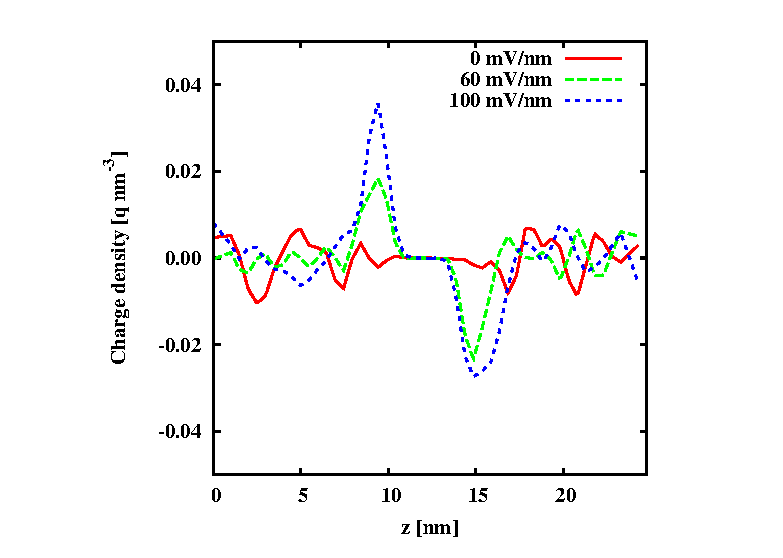
\includegraphics[width=.8\textwidth]{Figure1.eps}
\end{center}
\caption{Calculated free ion charge distribution in the $z$-direction demonstrates the build up of interfacial charge with the applied field increase - $0$, $60$ and $100$ $mV/nm$  }
\label{fig:nvt_charges_all_voltage}
\end{figure}

Averaging over time was performed over the last 2.5 $ns$ of the production run.
An external electric field with strengths up to $100\, mV/nm$ does not rupture the toluene film for  the duration of the $NVT$ simulation -  $5\, ns$. 
It should be noted that the  charge distribution $NVT$ obtained at the $120\, mV/nm$ field within time intervals less than $500\, ps$  shown in the Figure \ref{fig:120mV_0-05ns} feature on average the same patterns as the distribution computed   $100\, mV/nm$ field shown with a blue line in the Figure \ref{fig:nvt_charges_all_voltage}.\\
Electric discharge is initiated after the pore formation as it is seen in the Figure \ref{fig:diff_120mV_2-5ns}. After $2\, ns$, the accumulated interfacial charge is drained - no peaks in the charge distribution of the ruptured film. 

\begin{figure}[h]
\centering
\begin{subfigure}{.45\textwidth}
  \centering
  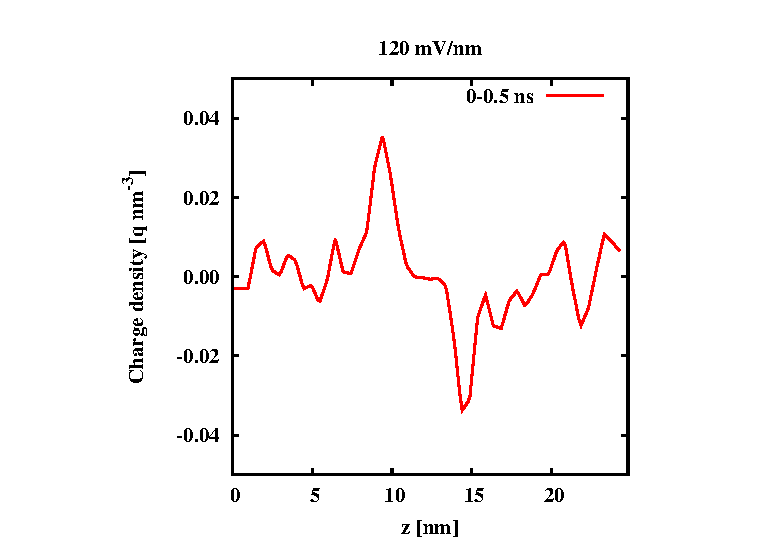
\includegraphics[width=\textwidth]{Figure2a.eps}
  \caption{Free ions charge distribution at $120\, mV/nm$ between $0 - 0.5\, ns$}
  \label{fig:120mV_0-05ns}
\end{subfigure}%
\begin{subfigure}{.45\textwidth}
  \centering
  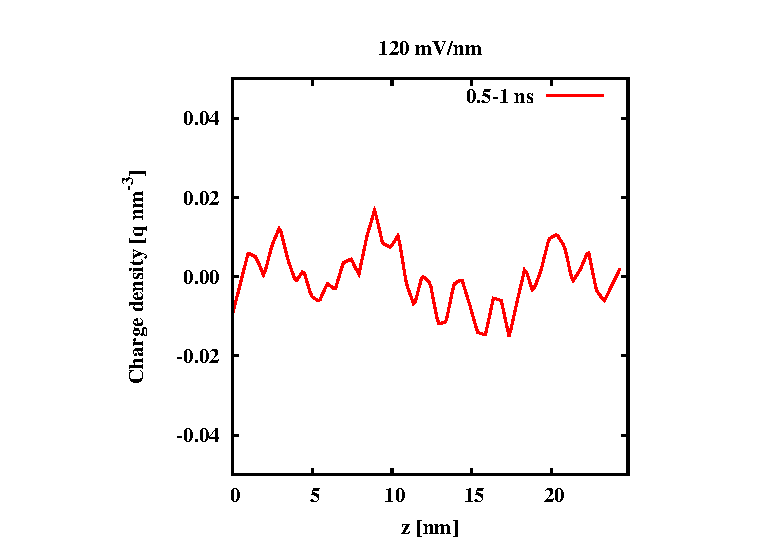
\includegraphics[width=\textwidth]{Figure2b.eps}
  \caption{Free ions charge distribution at $120\, mV/nm$ between $0.5 - 1\, ns$}
  \label{fig:120mV_05-1ns}
\end{subfigure}
%\vskip\baselineskip
\begin{subfigure}{.45\textwidth}
  \centering
  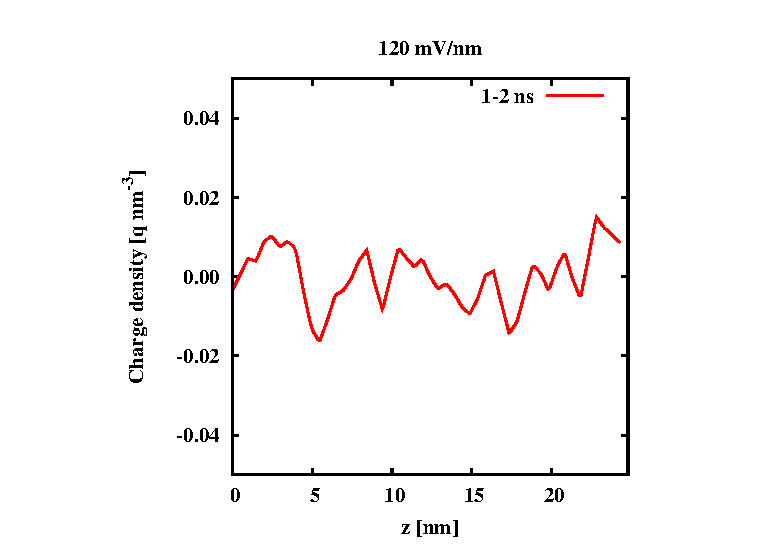
\includegraphics[width=\textwidth]{Figure2c.eps}
  \caption{Free ions charge distribution at $120\, mV/nm$ between $1 - 2\, ns$}
  \label{fig:diff_120mV_1-2ns}
\end{subfigure}
\begin{subfigure}{.45\textwidth}
  \centering
  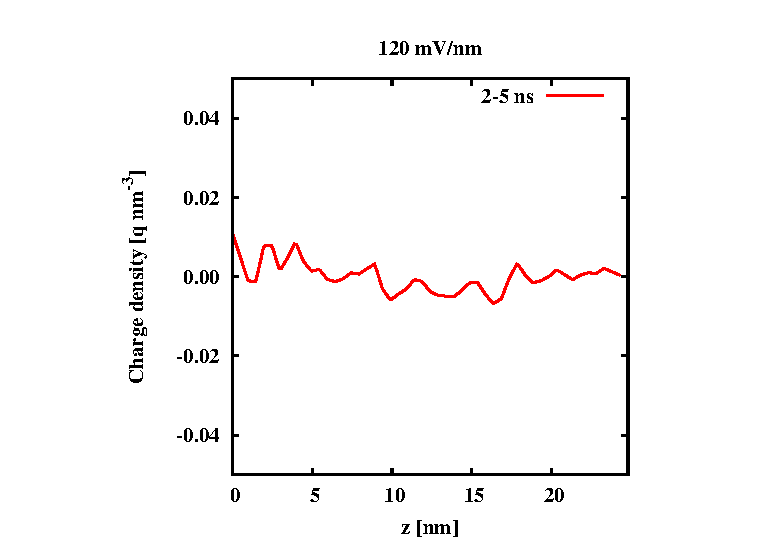
\includegraphics[width=\textwidth]{Figure2d.eps}
  \caption{Free ions charge distribution at $120\, mV/nm$ between $2 - 5\, ns$}
  \label{fig:diff_120mV_2-5ns}
\end{subfigure}
\caption{Free ions charge distribution at $120\, mV/nm$}
\label{fig:nvt_charge_distrib_120mV}
\end{figure}

\begin{figure}[h]
\centering
\begin{subfigure}{.45\textwidth}
  \centering
  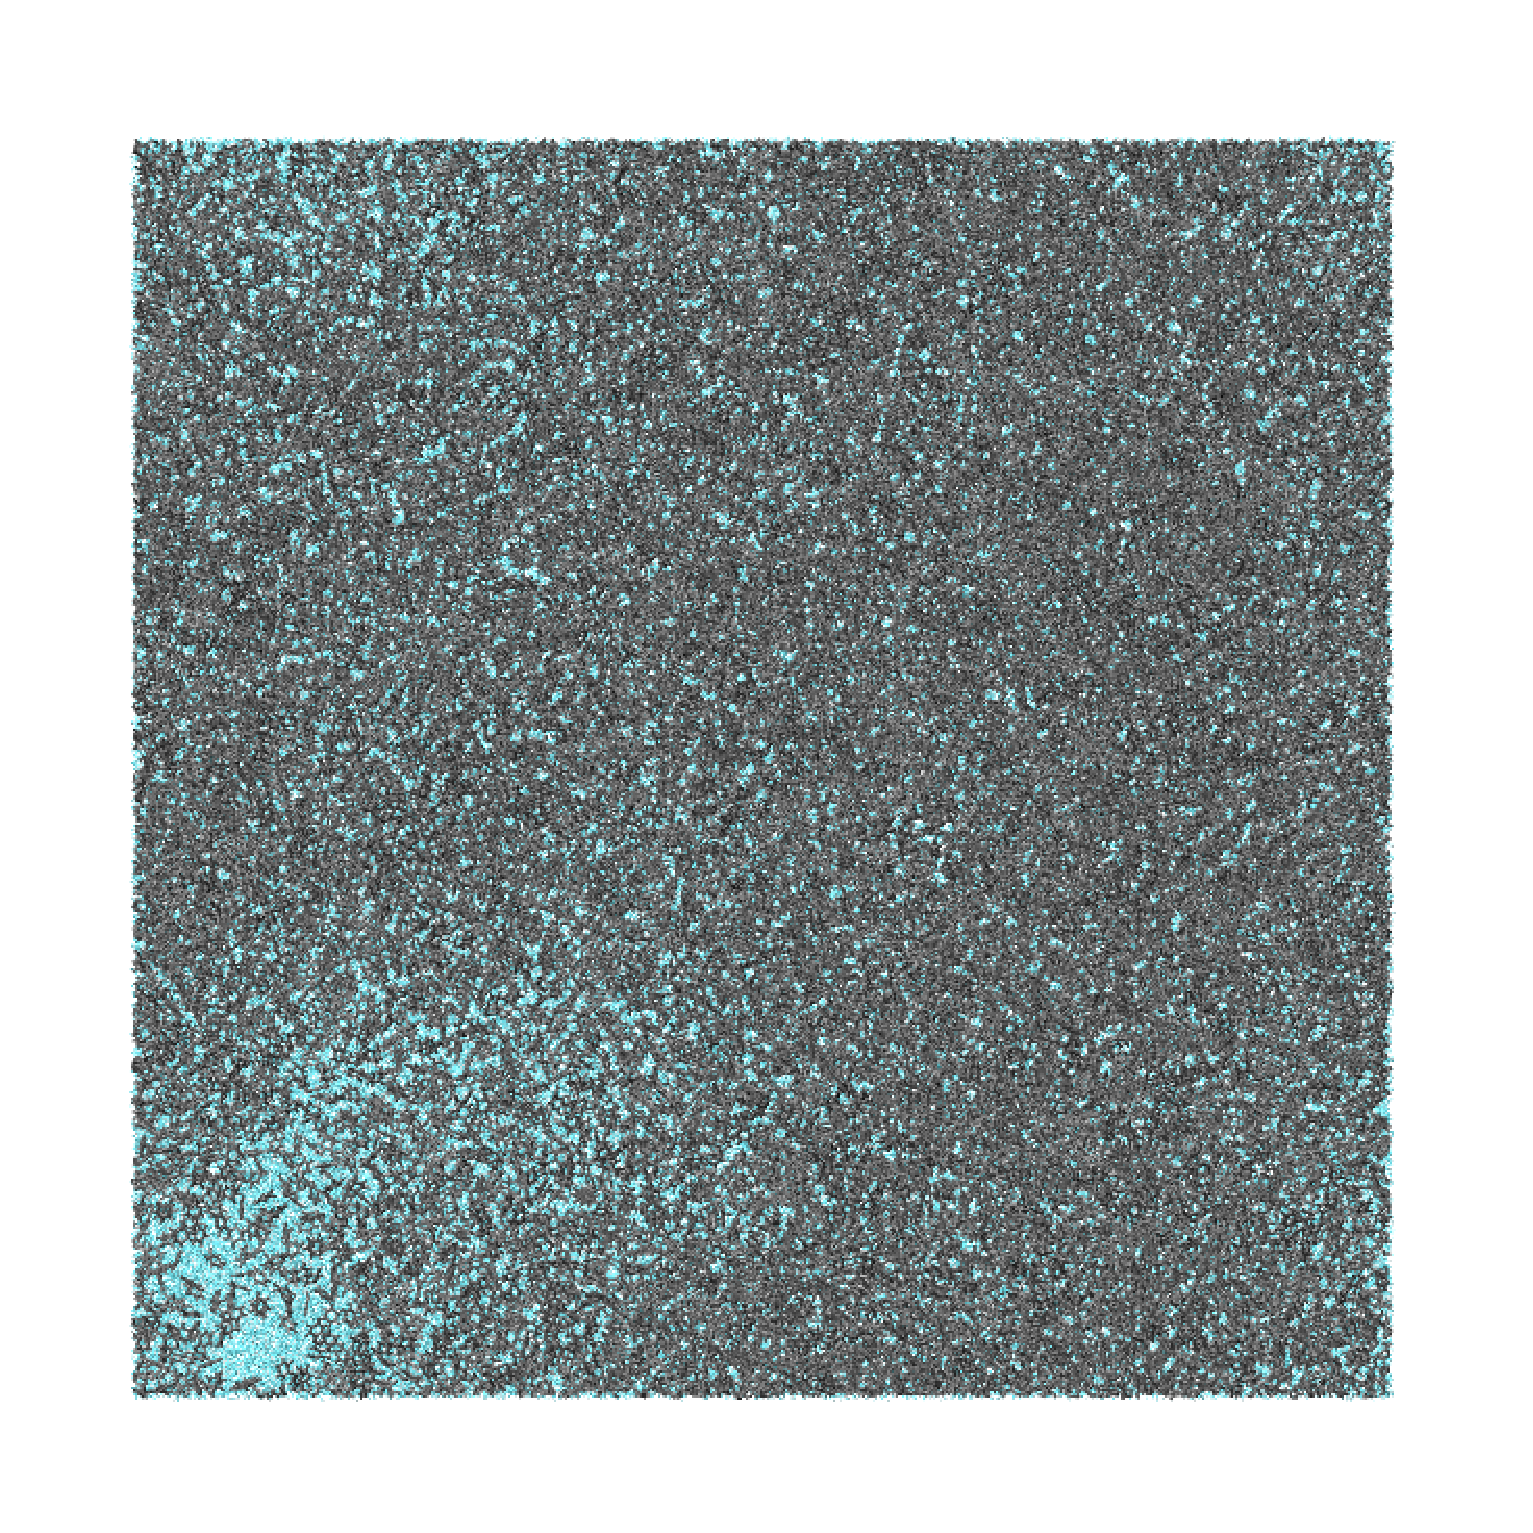
\includegraphics[width=.8\textwidth]{Figure3a.eps}
  \caption{$500\, ps$}
  \label{fig:top_view_500ps}
\end{subfigure}%
\begin{subfigure}{.45\textwidth}
  \centering
  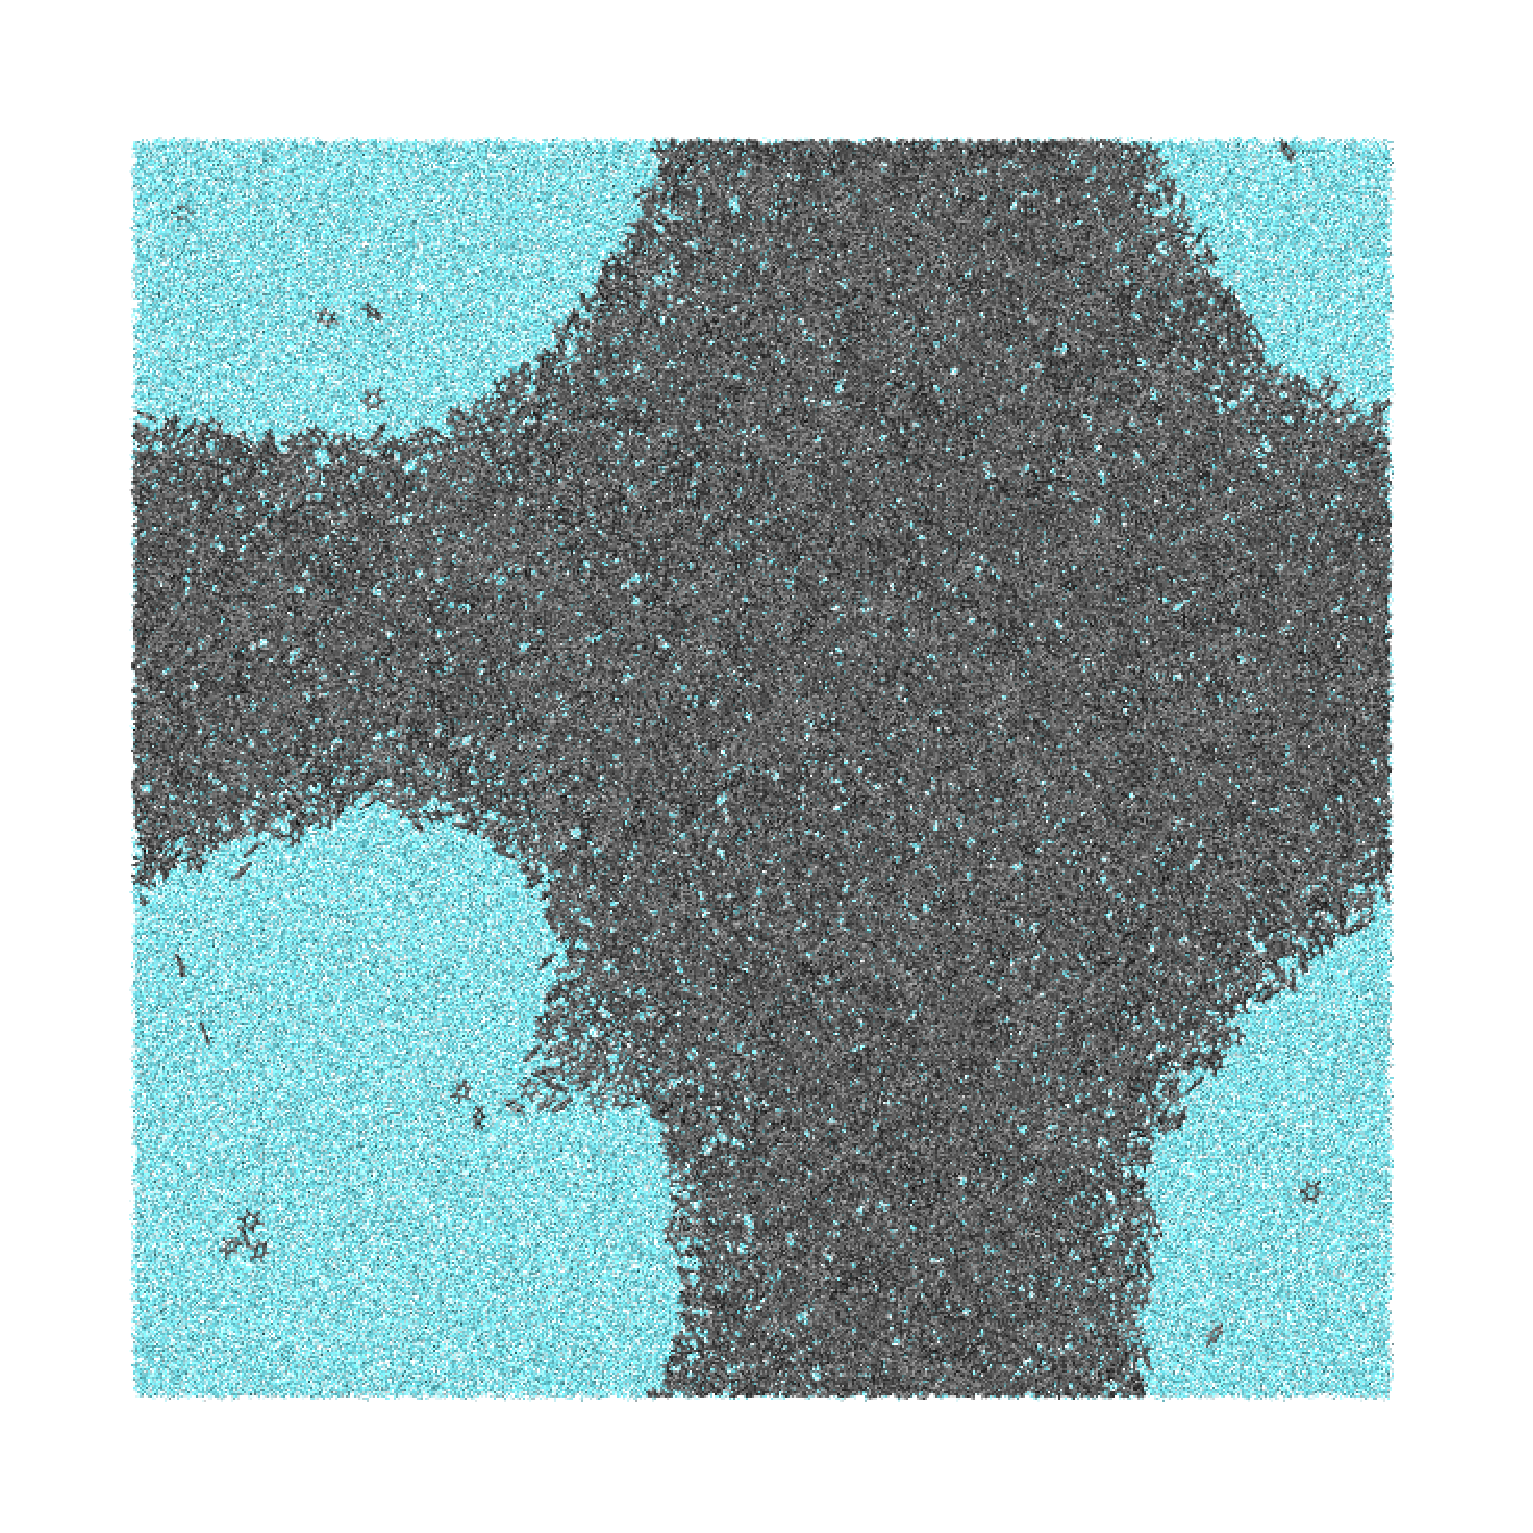
\includegraphics[width=.8\textwidth]{Figure3b.eps}
  \caption{$700\, ps$}
  \label{fig:top_view_700ps}
\end{subfigure}
%\vskip\baselineskip
\begin{subfigure}{.45\textwidth}
  \centering
  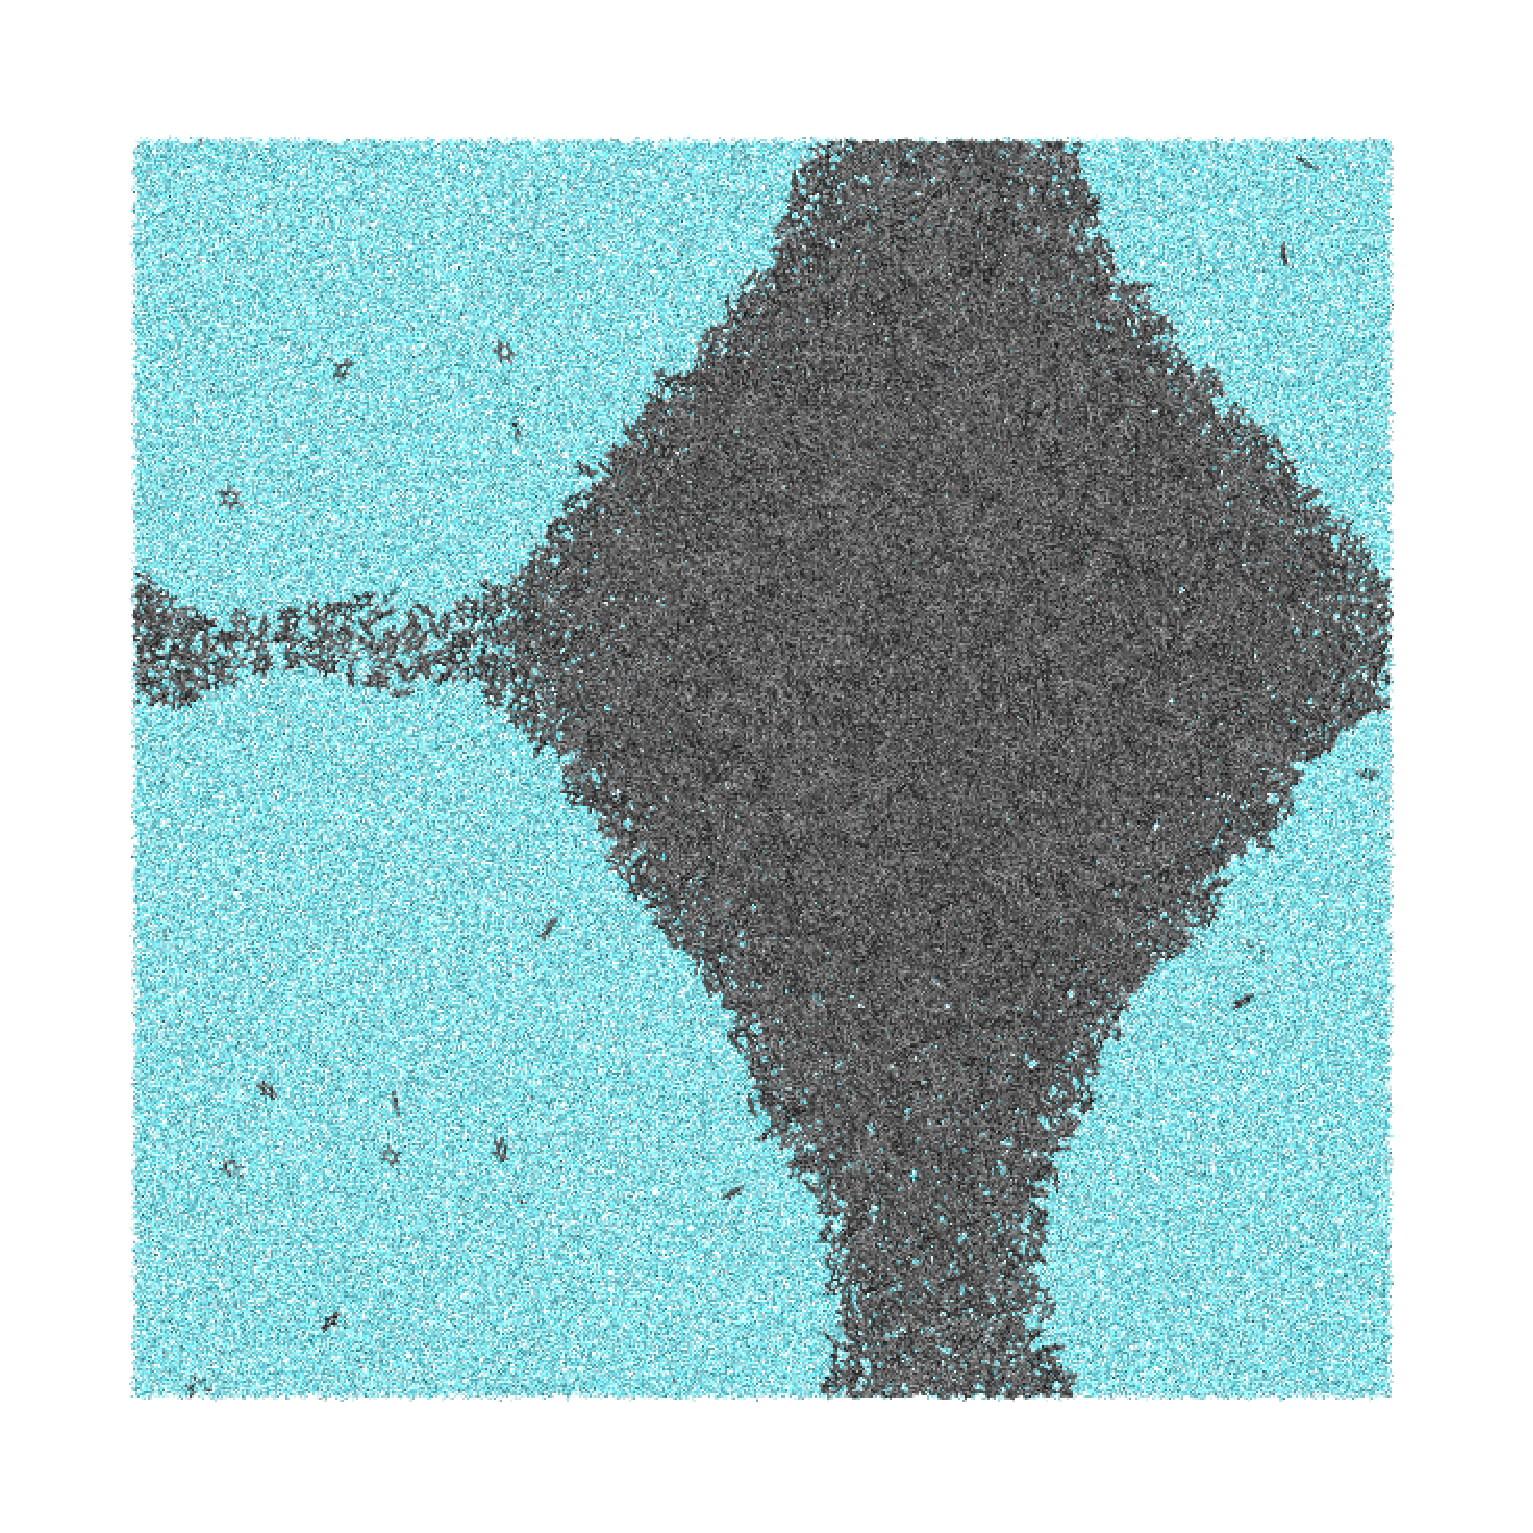
\includegraphics[width=.8\textwidth]{Figure3c.eps}
  \caption{$1500\, ps$}
  \label{fig:top_view_1500ps}
\end{subfigure}
\begin{subfigure}{.45\textwidth}
  \centering
  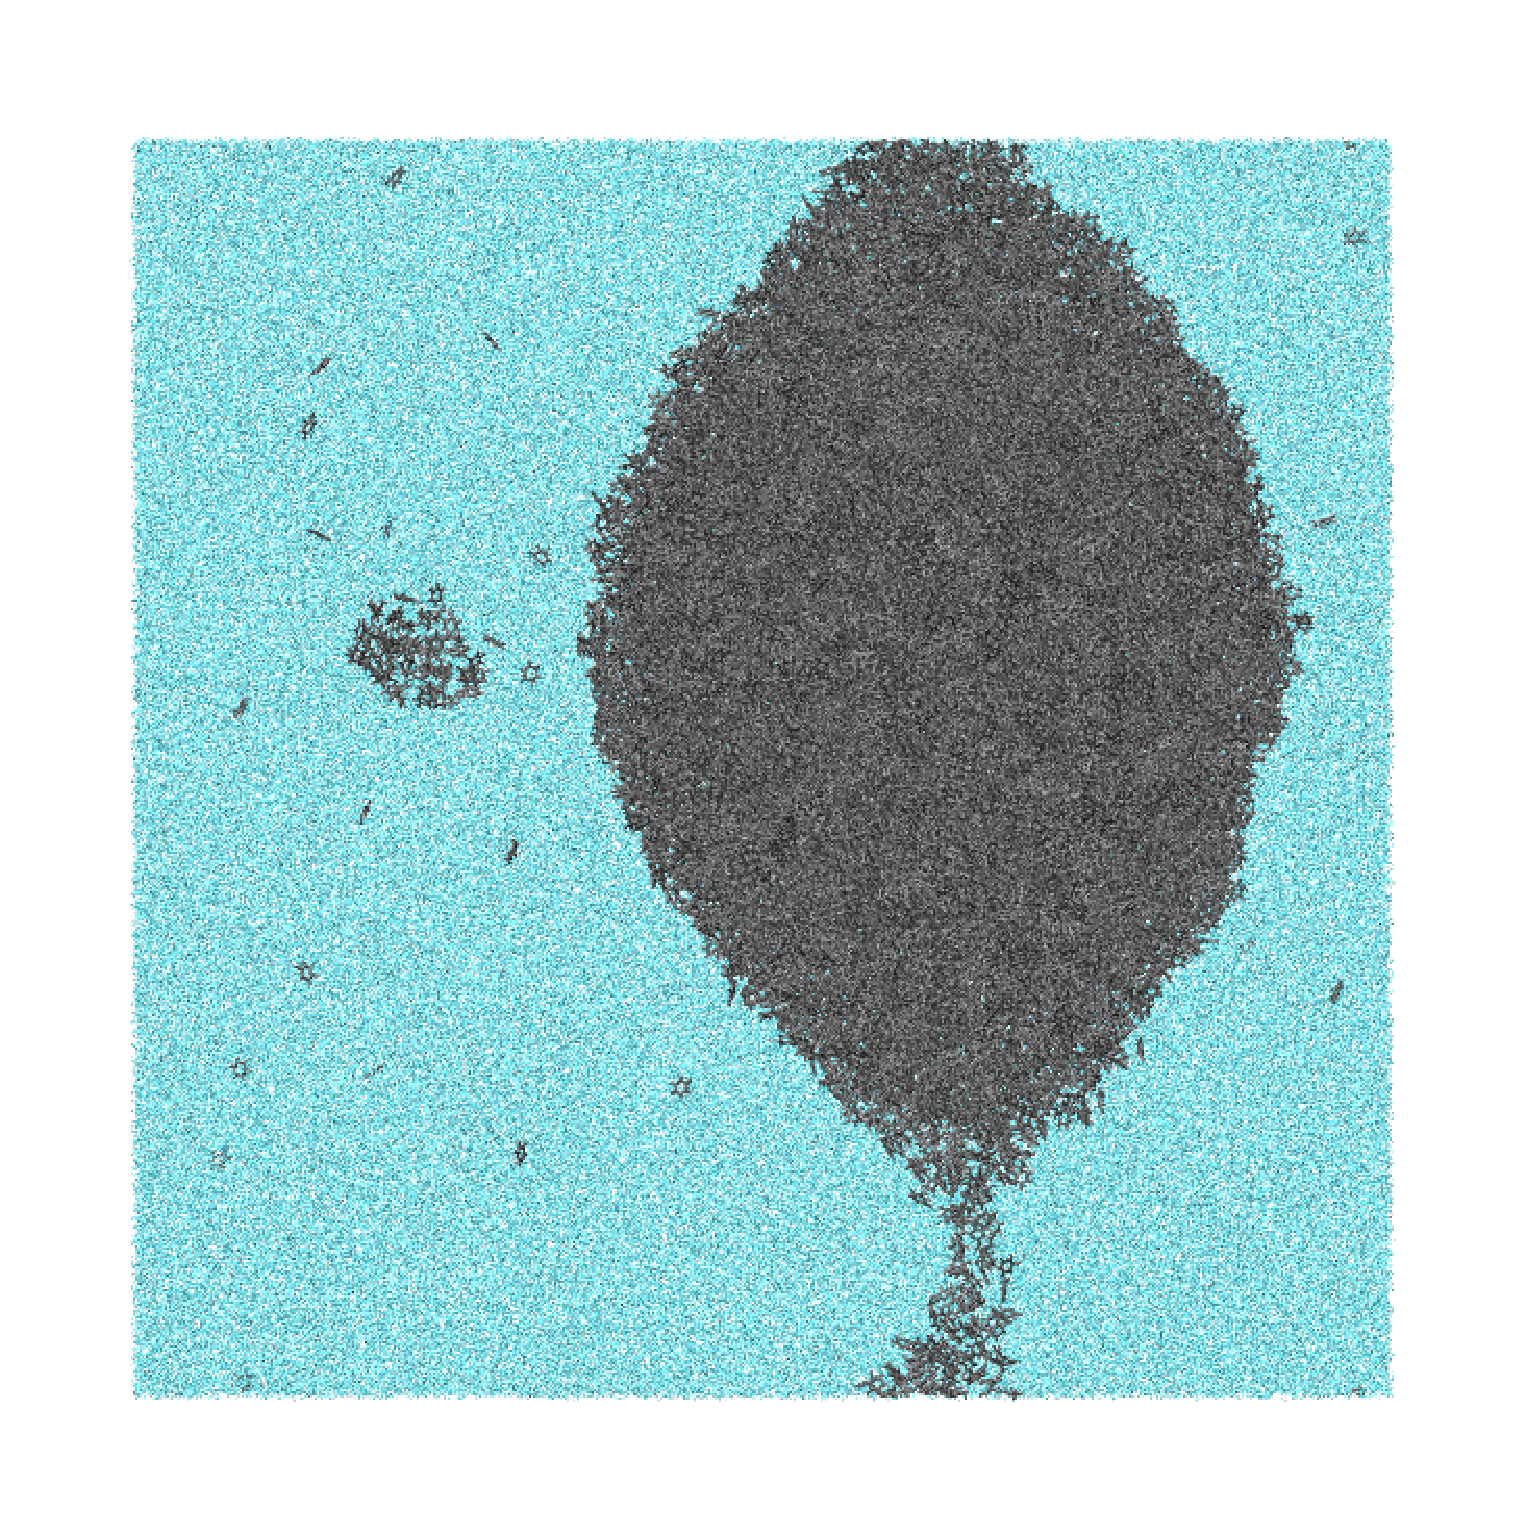
\includegraphics[width=.8\textwidth]{Figure3d.eps}
  \caption{$2000\, ps$}
  \label{fig:top_view_2000ps}
\end{subfigure}
\caption{Top view snapshot of time evolution of film area at applied external electric field of $120\, mV/nm$}
\label{fig:film_rupture_nvt}
\end{figure}



\subsection{$NVT$ simulation - film rupture mechanism}
When the electric field is set to $120\, mV/nm$ a pore is formed in  the film after $500\, ps$. It is observed that the pore expands along the simulation box over time. The time evolution of the pore formation is shown in Figure \ref{fig:film_rupture_nvt} for the time between  $500\, ps$ and $2000\ ps$. The pore is seen as a light spot in Figure \ref{fig:top_view_500ps} at $500\, ps$. When the pore is wide enough water molecules fill in the pore area, seen as a bluish background in the Figure \ref{fig:top_view_700ps} at $700\, ps$. By observing the pore evolution in the toluene film, the time of the complete film rupture (formation of toluene drop)  can be determined.
  
%Formation of other three rupturing places in form of light spots is due to applied periodic boundary conditions. In the Figure \ref{fig:nvt_side_view_film_rupture} the side view of the simulation box is depicted. 

\begin{figure}[h]
\centering
\begin{subfigure}{.32\textwidth}
  \centering
  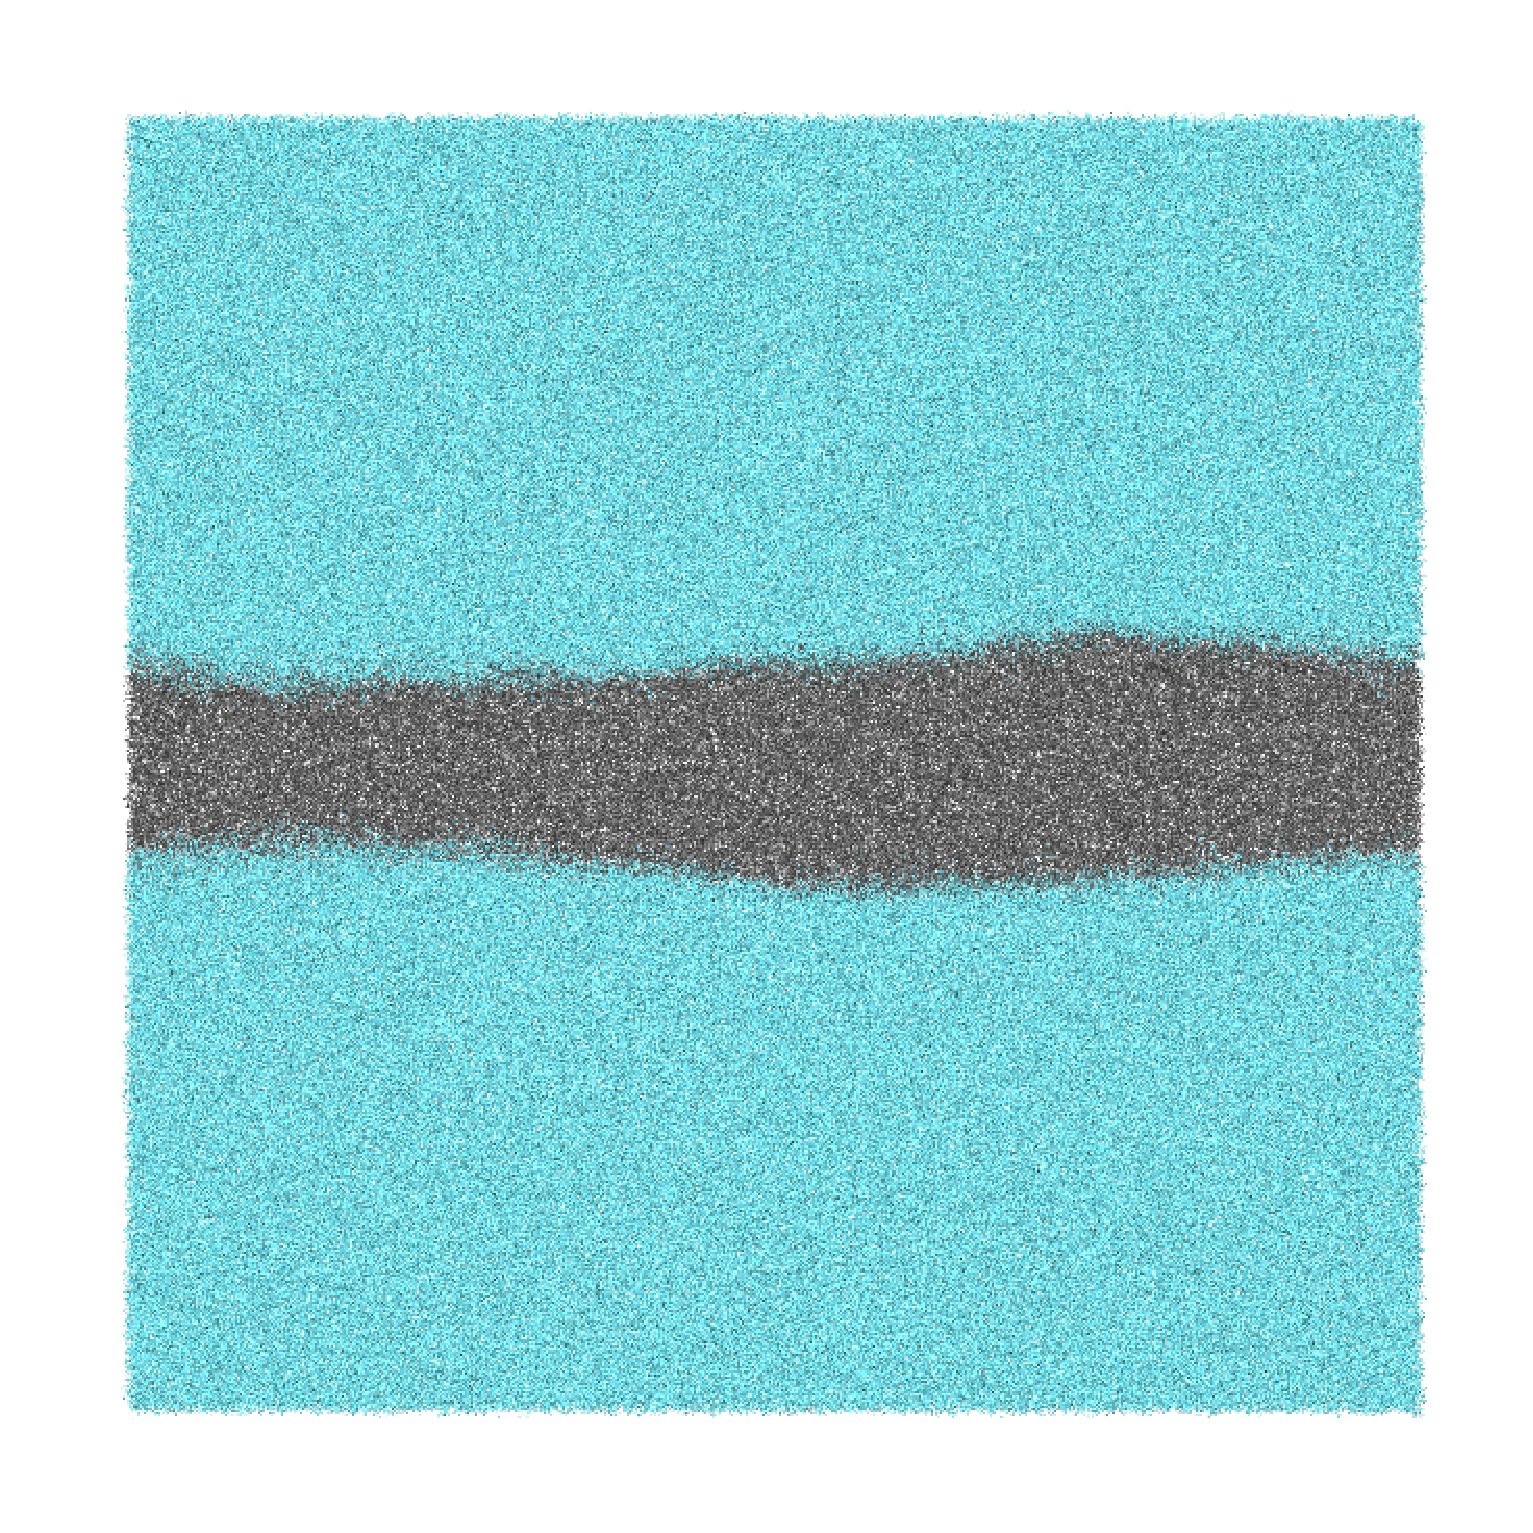
\includegraphics[width=\linewidth]{Figure4a.eps}
  \caption{$100\, ps$}
  \label{fig:side_view_100ps}
\end{subfigure}%
\begin{subfigure}{.32\textwidth}
  \centering
  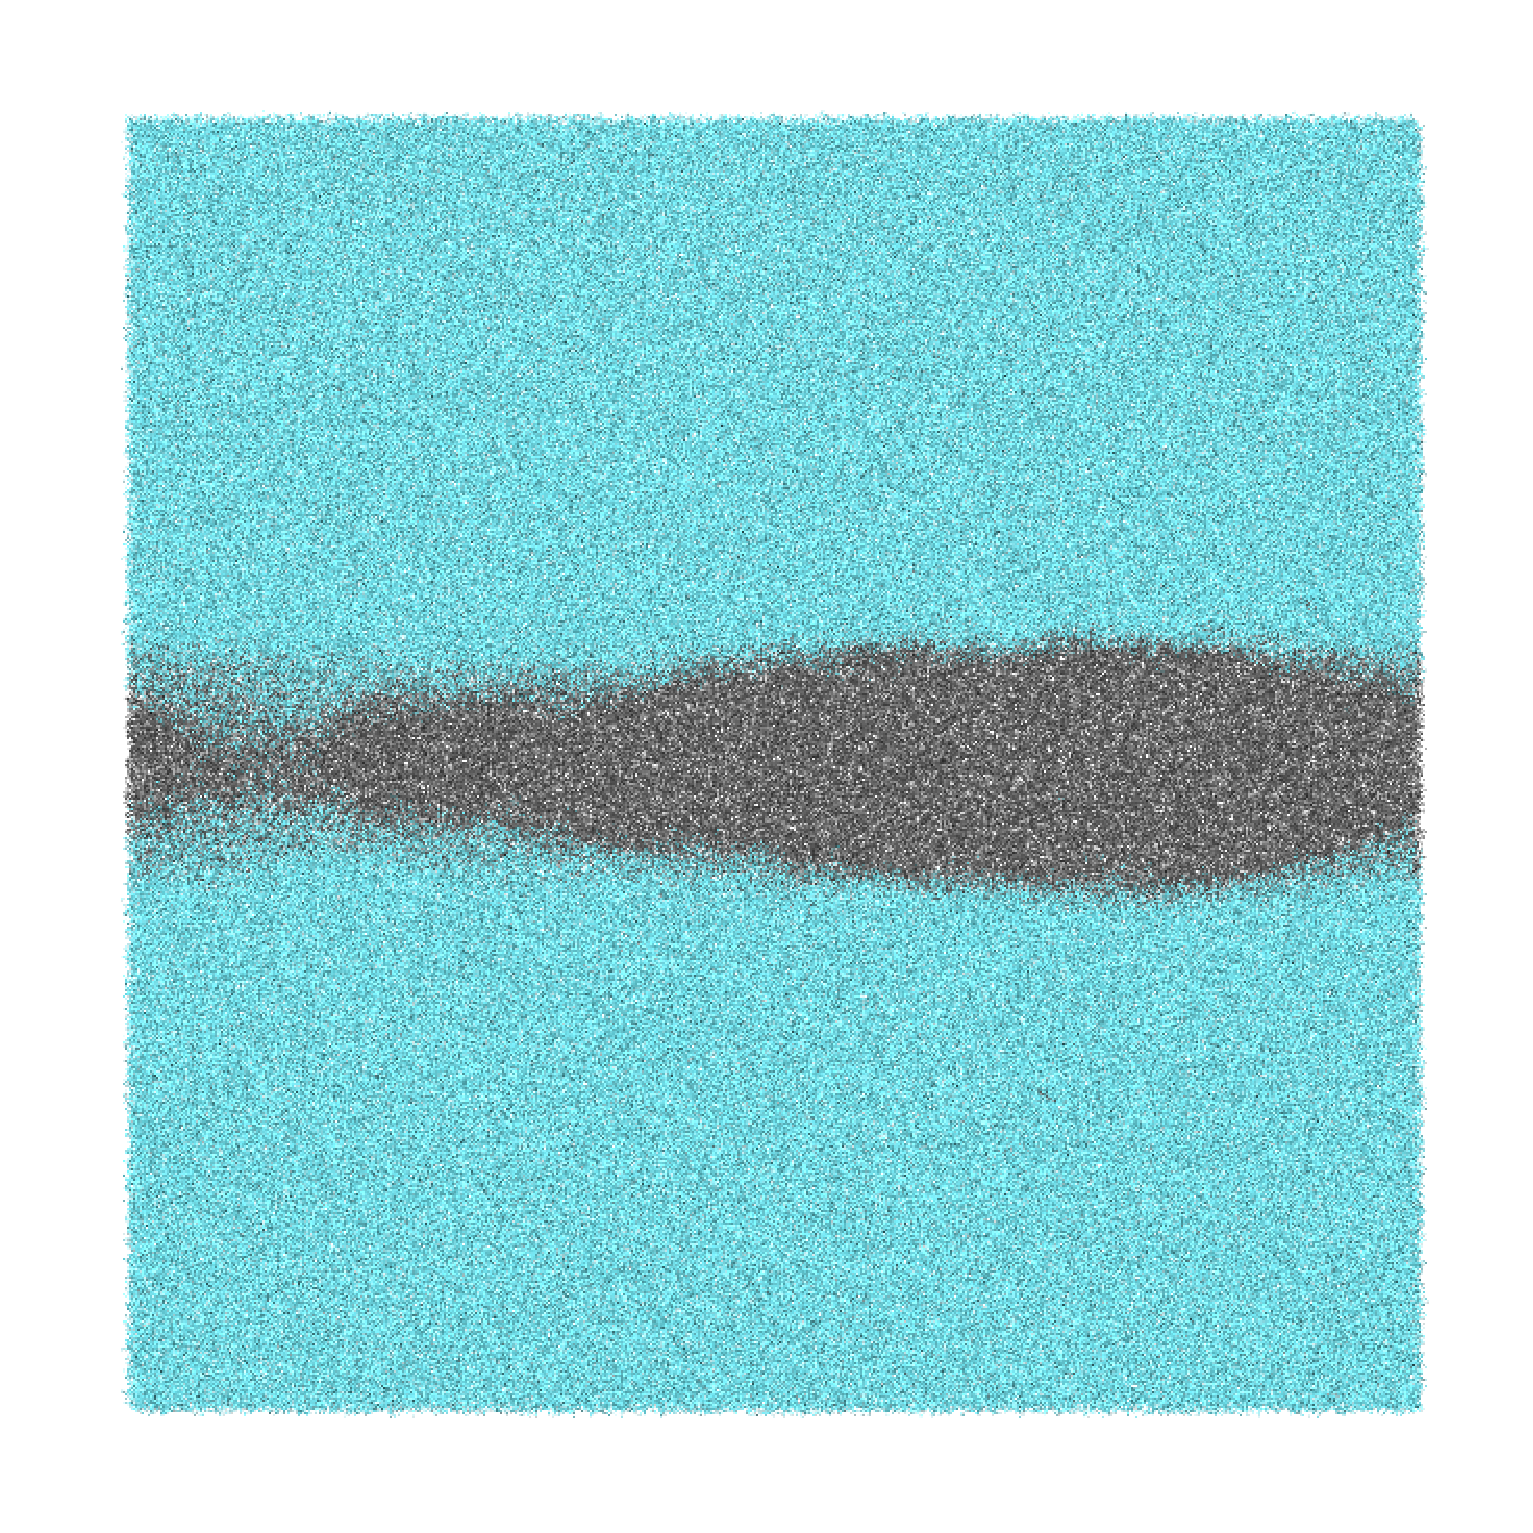
\includegraphics[width=\linewidth]{Figure4b.eps}
  \caption{$500\, ps$}
  \label{fig:side_view_500ps}
\end{subfigure}
\begin{subfigure}{.32\textwidth}%
  \centering
  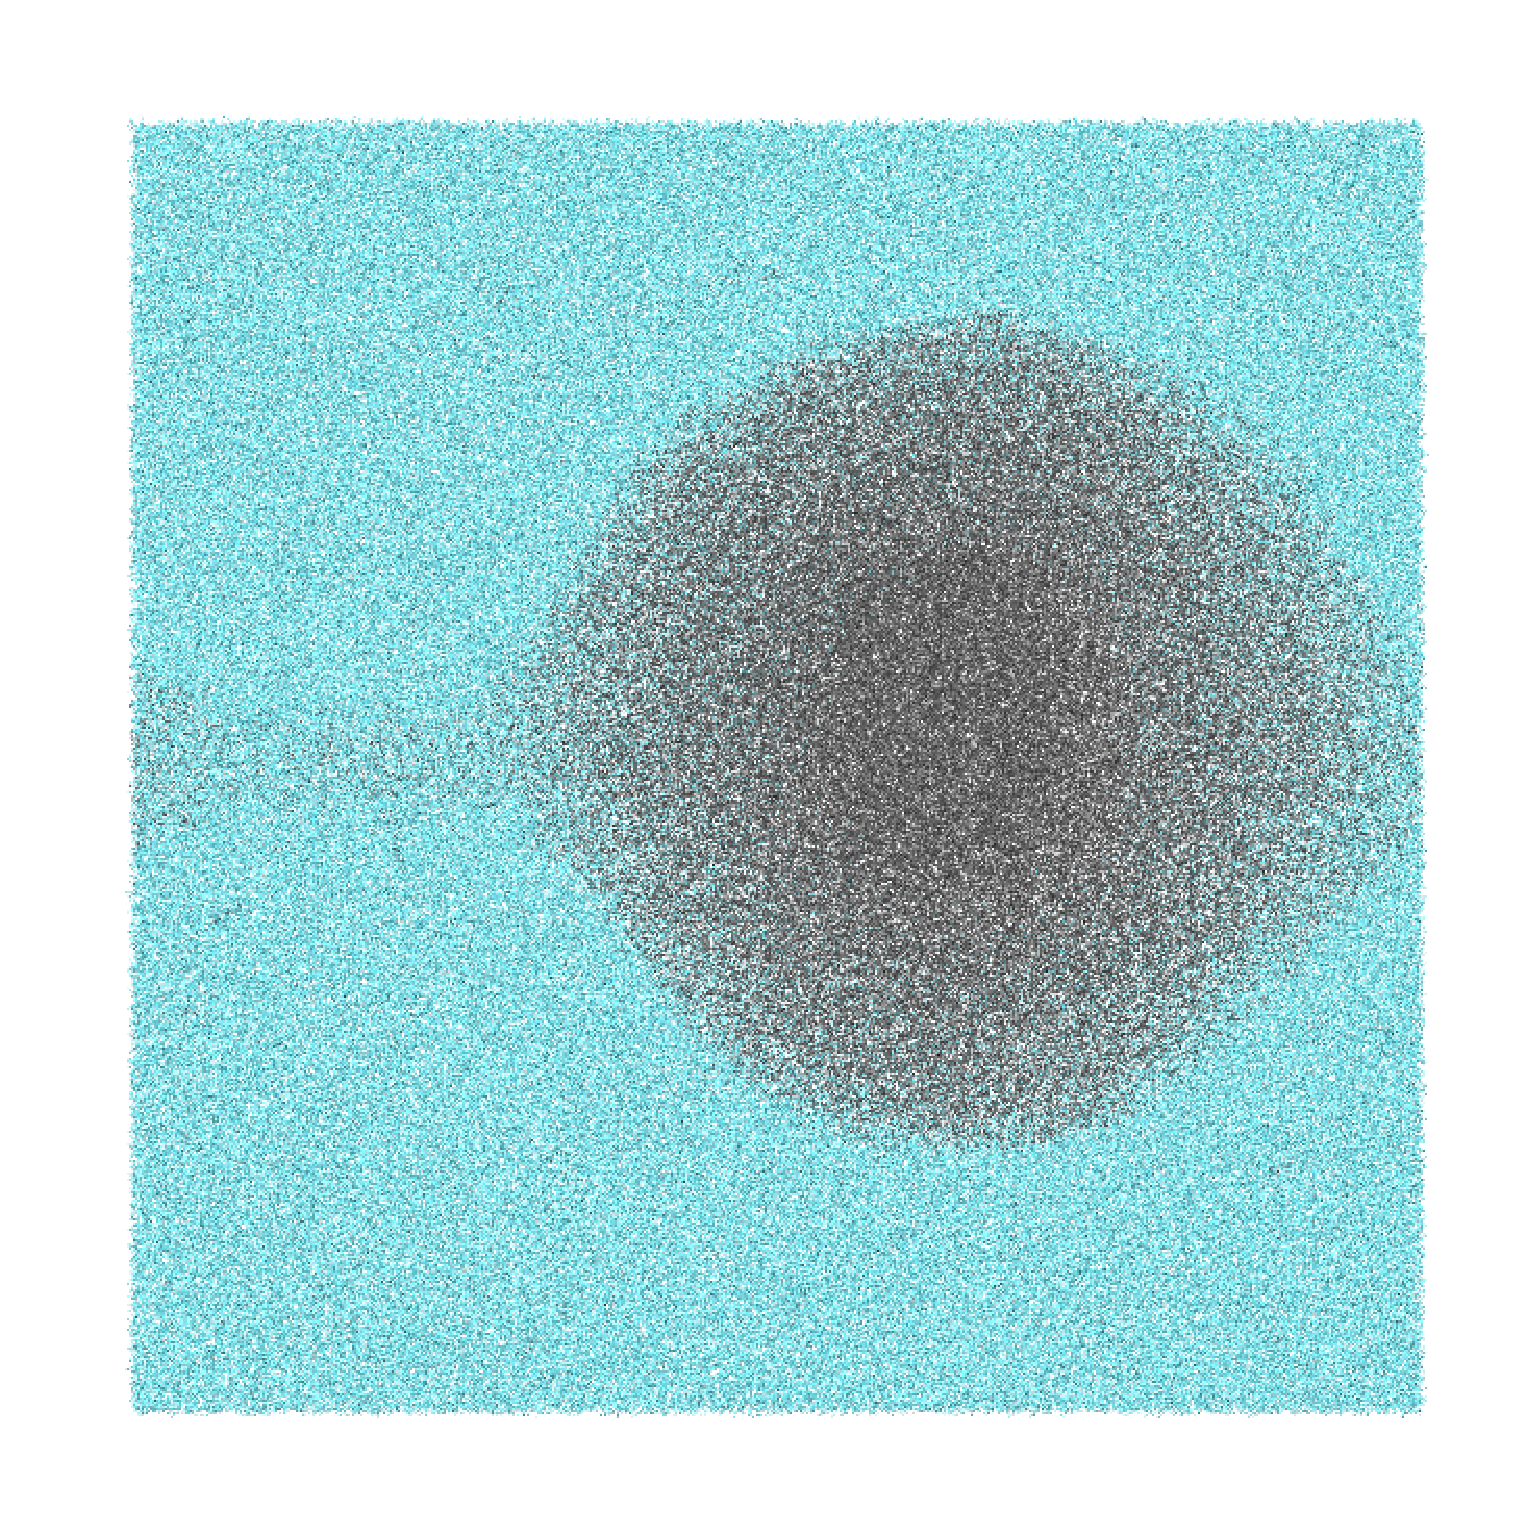
\includegraphics[width=\linewidth]{Figure4c.eps}
  \caption{$2000\, ps$}
  \label{fig:side_view_1500ps}
\end{subfigure}
\caption{Side view snapshots for the $120\, mV/nm$ external electric field applied  perpendicularly to the toluene film:  (a) the film profile after $100\, ps$; (b) startup of rupturing of the thinnest part of the film - between $400\, ps$ and $500\, ps$;  (c) breakdown of the film and formation of a toluene drop at about $2000\, ps$}.
\label{fig:nvt_side_view_film_rupture}
\end{figure}

Inspection of the thickness profile at $120 mV/nm$ reveals existence of a dimple inside the toluene film (Figure \ref{fig:side_view_100ps}) prior to the film rupture.The role of the non-homogeneity has been widely reported in thin liquid film literature since 1941 \cite{Landau_1941}. 

Our simulations demonstrate that a non-homogeneous film ruptures at its thinnest place because the electric field strength is the highest there. In other words, the biconcave region of the film interface is subjected to a higher\textendash than\textendash average electrostatic pressure and therefore is a preferred site for the film rupture and nano\textendash pore formation.\\
% The accumulation of ions increases the electrostatic pressure.


\subsection{$NVT$ simulation - the film structure}
The charge density  of free ions, water, and toluene molecules in the $z$-direction can be observed in the Figure \ref{fig:nvt_all_distributions}. The  figure illustrates the structure of the toluene film surrounded by aqueous electrolyte solution at $0$, $60$, $100$ and $120$ $mV/nm$ electric field strengths. For the latter case the density was averaged over the first $0.5\, ns$ of simulation, i.e. before the startup of the rupturing process. The part of the  film that contains only toluene molecules is called toluene {\it core}, {\it bulk} water phase is that part of the film, where the density of water molecules is maximal.

The core thickness was estimated using a double\textendash sigmoid function (Equation \ref{eq:double_sigmoid}) at $99\%$ of the plateau height $h$, where $x_0$, $x_1$ being the left and the right half-height respectively, $a$ is the steepness of the sigmoid:
\begin{equation}
f(x;x_0, x_1, a, h) = h\bigg(1 - \frac{1}{1 + \exp^{-a(x-x_1)}}\bigg) \frac{1}{1 + \exp^{-a(x-x_0)}}
\label{eq:double_sigmoid}
\end{equation}

At no applied field, Figure \ref{fig:nvt_dens_dist_0mV} there exists a pure toluene core of $2.6\, nm$ thickness, which is surrounded by two interfacial layers formed by mixing toluene and water interfacial layers. In the toluene interfacial layer, the concentration of toluene molecules decreases in the direction from the pure toluene core towards the bulk water phases, eventually reaching zero concentration. Respectively, in the aqueous interfacial layer, the concentration of water molecules decreases towards the toluene core. Toluene\textendash water mixed layer is $1.4\, nm$ thick, which is estimated as the distance where the toluene density in $z$-direction drops from $99\, \%$ to $1\, \%$ from the plateau height $h$. The bulk aqueous phases contain $Na^+$ and $Cl^-$ ions. The density profiles show that ions penetrate the mixed interfacial layers that border the toluene core. 
Thicknesses of the film core and the interfacial layer are shown in the Table \ref{table:nvt_film_thickness}.

\begin{center}
\begin{table}[ht]
\centering
\begin{tabular}{|c|c|c|c|c|}
\hline
%\backslashbox{layer}{applied field} 
applied field           &$0\, mV/nm$   &$60\, mV/nm$   &$100\, mV/nm$   &$120\, mV/nm$ \\ \hline
toluene core [nm]       &$2.6$         &$2.4$          &$2.0$           &$1.8$   \\ \hline
interfacial layer [nm]  &$1.4$         &$1.7$          &$2.1$           &$2.5$    \\ \hline
total toluene layer [nm]  &$5.4$         &$5.8$          &$6.2$           &$6.8$    \\ \hline
\end{tabular}
\caption{Film thickness at different strength of the applied electric field in NVT ensemble }
\label{table:nvt_film_thickness}
\end{table}
\end{center}


The Figure \ref{fig:nvt_dens_dist_60mV} shows that application of $60\, mV/nm$ field leads to build-up of accumulated positive charges on one side of the toluene film and negative charges on the other side. The peaks of accumulated charges are  situated at the boundary between bulk water and interfacial aqueous layer. In the direction towards toluene core, the concentration of ions decreases  and reaches zero at the toluene core. Ions penetrate only the mixed interfacial region, which is due to the formation of hydration shells. The Figure \ref{fig:nvt_dens_dist_100mV} reveals that field increase up to $100\, mV/nm$ is followed by accumulation of more charges, bringing enough attractive force that leads to thinning of the pure toluene core by $0.6\, nm$ down to $2.0\, nm$, while the thickness of the interfacial layers of toluene and water increases by $0.7\, nm$. 
%Furthermore the peak position of the accumulated charge stays at the end of the bulk water region but the spread of the charge distribution increase due to a thicker mixed region. 
%Furthermore, the penetration of ions in the direction from the accumulation lines towards mixed region increases by $0.5\, nm$, reaching almost the end of that region. 
%Further on, ions do not intervene in the boundary layer, where only toluene molecules are present. 
A possible hypothesis is that the increased electrical compression reshapes the film topography making it a high amplitude rugged surface and the interfacial layer becomes thicker.
%We can speculate that during increased electrical compression the toluene molecules escape from the toluene core and enter the interfacial toluene layer thus expanding its width. 
%The other possibility that toluene molecules in the core get closer to each other during the compression, should lead to increase of the density of the core. However, this is not the case since Figure \ref{fig:nvt_all_distributions} do not show change of core density. 
The Figure \ref{fig:nvt_dens_dist_120mV} depicts the film structure (profile) at $120\, mV/nm$ and data are averaged over the time interval of $500\, ps$. This  is the moment ($500\, ps$) just before the rupturing process takes place. 


\begin{figure}[h]
\centering
\begin{subfigure}{.45\textwidth}
  \centering
  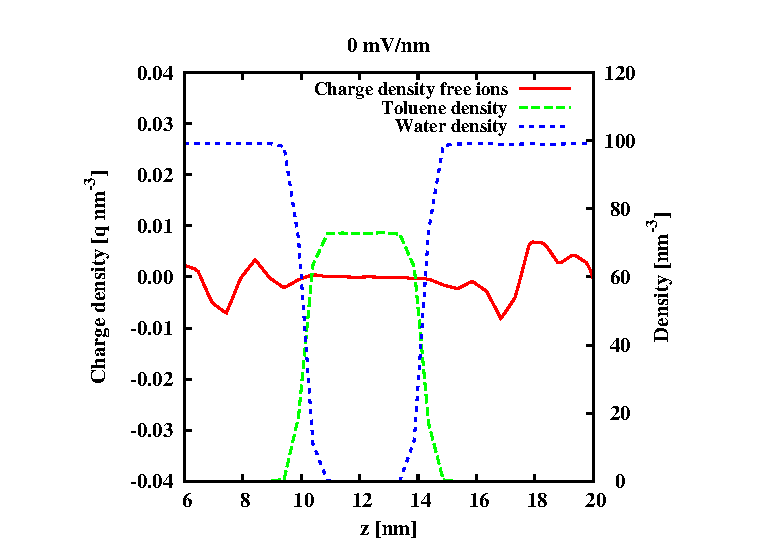
\includegraphics[width=\textwidth]{density_prot_sol_charge_na_cl_0mV.eps}
  \caption{Density distribution at external electric field $0 mV/nm$}
  \label{fig:nvt_dens_dist_0mV}
\end{subfigure}%
\begin{subfigure}{.45\textwidth}
  \centering
  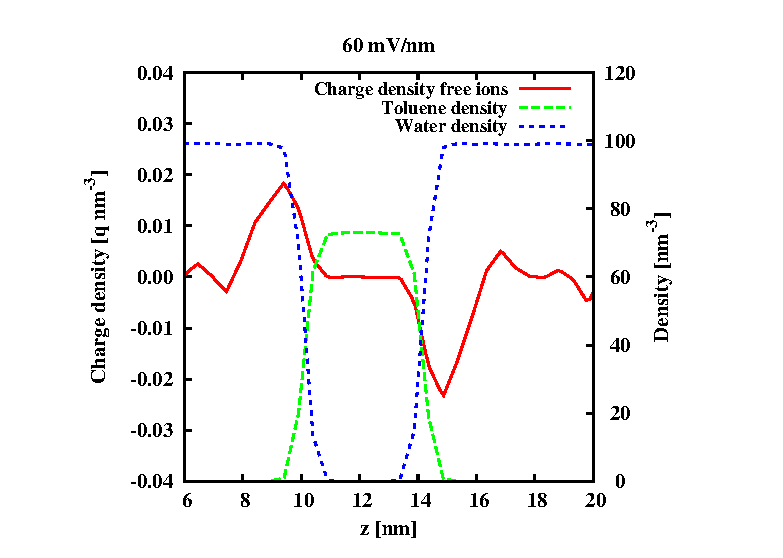
\includegraphics[width=\textwidth]{density_prot_sol_charge_na_cl_60mV.eps}
  \caption{Density distribution at external electric field $60 mV/nm$}
  \label{fig:nvt_dens_dist_60mV}
\end{subfigure}
%\vskip\baselineskip
\begin{subfigure}{.45\textwidth}
  \centering
  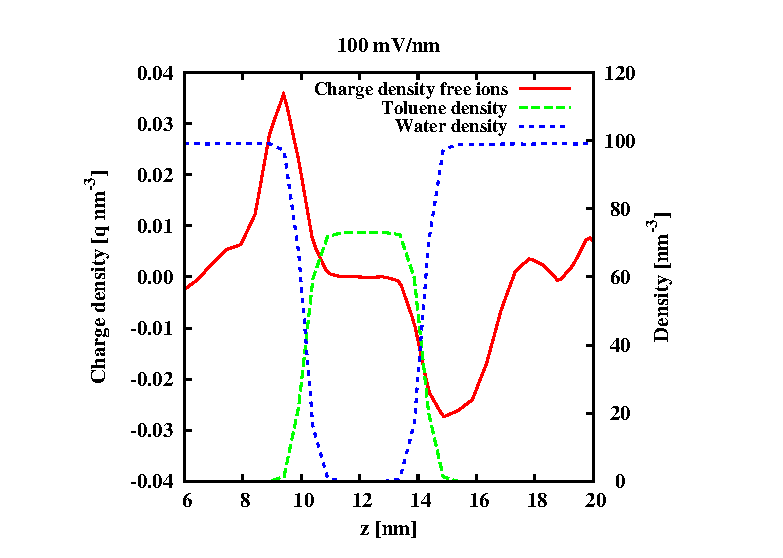
\includegraphics[width=\textwidth]{density_prot_sol_charge_na_cl_100mV.eps}
  \caption{Density distribution at external electric field $100 mV/nm$}
  \label{fig:nvt_dens_dist_100mV}
\end{subfigure}
\begin{subfigure}{.45\textwidth}
  \centering
  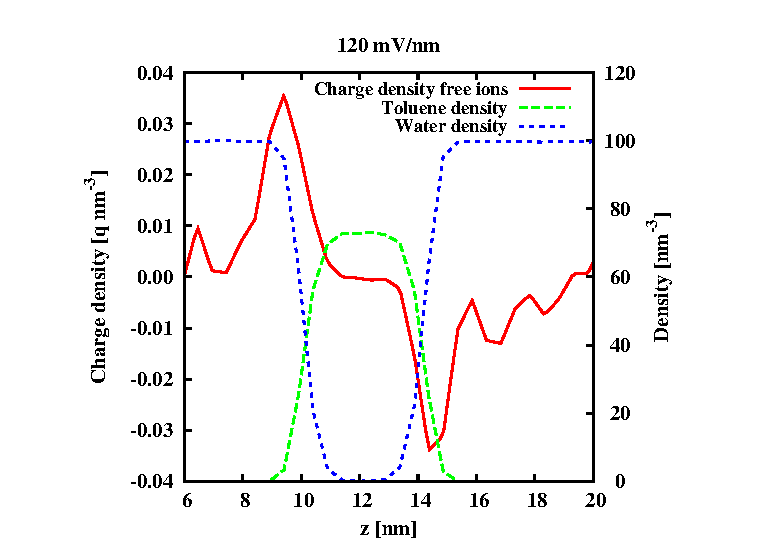
\includegraphics[width=\textwidth]{density_prot_sol_charge_na_cl_120mV.eps}
  \caption{Density distribution at external electric field $120 mV/nm$}
  \label{fig:nvt_dens_dist_120mV}
\end{subfigure}
\caption{Density distribution of free ions (red), toluene (green) and water molecules (blue) at different external electric fields in NVT ensemble}
\label{fig:nvt_all_distributions}
\end{figure}

The increase of potential from $100$ to $120\, mV/nm$ leads to additional thinning of the toluene core down to $1.8\, nm$. The thickness of interfacial layers of toluene and water increases by $0.4\, nm$. 
%It is worthwhile mentioning though, that the thickness of the ionic interfacial layer on the left side, where accumulation of $Na^+$ ions occurs, is twice larger than the thickness of ionic layer on the right side ($Cl^-$ ions). It is a bit surprising that at $120\, mV/nm$ ionic and aqueous interfacial layers do not approach any closer the toluene core, in comparison with $100\, mV/nm$. 



\subsection{$NPT$ simulation - the film structure}
%The charge density distributions of the free ions is given in the Figure \ref{fig:npt_charges_all_voltage} for the case of a $NPT$ ensemble with a constant surface tension. 
%%Toluene core appears to be $0.5\, nm$ thinner than in NVT simulation,
%Although there is no significant difference between thicknesses of the toluene core in $NVT$ and $NPT$ ensembles at $0\, mV/nm$, the interfacial layer is thicker 
%by $0.4\, nm$ 
%in the case of the $NPT$ ensemble.
%%Relatively \underline{small} (*$5.10^7$ V/m you should compare with the atomic field) 
%Thicknesses of different layers were again determined by using the double\textendash sigmoid Equation \ref{eq:double_sigmoid}.
%Field strength of 
%Relatively small increase of field strength up%
% $50\, mV/nm$ (Figure \ref{fig:npt_dens_dist_50mV}) in the $NPT$ ensemble already squeezes the toluene core (Table \ref{table:npt_film_thickness}). In comparison with the NVT case, a $60\, mV/nm$  field produces a smaller change in the toluene core. Thickness of the boundary layers of toluene and water appear to be higher in the NPT ensemble.   

In this section, the results from $NPT$ canonical ensemble simulation are presented. 
%{\color{red} 
The charge  build\textendash up is plotted in the Figure \ref{fig:npt_charges_all_voltage}.
The Figure \ref{fig:npt_all_distributions} depicts the charge build-up at $0$, $25\, mV/nm$,  and $50\, mV/nm$. As in the NVT case, at zero external field no peak formation is observed on both sides of ionic line that exhibits zero-charge density. At $25\, mV/nm$ such formation already takes place and becomes much pronounced at $50$ and $75\, mV/nm$ (Figure \ref{fig:npt_dens_dist_75mV}).  Film rupture occurs at a much lower electric field strength ($75\,  mV/nm$) compared to the NVT simulation ($120\, mV/nm$). Film rupture occurs at a much lower electric field strength ($75\, mV/nm$) compared to the NVT simulation ($120\, mV/nm$). The information regarding the thickness of the toluene core, boundary layers and the total film are summarized in Table \ref{table:npt_film_thickness}. The thickness of different layers were again determined by using the double\textendash sigmoid formula in Equation \ref{eq:double_sigmoid}. At no applied field, the toluene core has the same thickness as in the NVT case. However, the difference between the two simulations is revealed in the size of the mixed boundary zone, being larger for the NPT ensemble. Increase of the electric field, as in the NVT case, again leads to the thinning of the toluene core and to the expansion of the boundary layers. However, at $50\, mV/nm$ (NPT) there is a bit higher thinning of the core, compared to $60\, mV/nm$ (NVT), despite of the lower applied field. This observation, together with the obtained lower critical field could suggest enhanced development of instability in the NPT simulation. It should be noted that in both simulations at the  critical field  the core has the same thickness instants before the film rupture.  Moreover, at that critical field the thickness of the boundary layers and of the total layer are almost identical in both $NVT$ and $NPT$ ensembles.
\begin{center}
\begin{table}[ht]
\centering
\begin{tabular}{|c|c|c|c|}
\hline
%\backslashbox{layer}{applied field} 
applied field           &$0\, mV/nm$   &$50\, mV/nm$   &$75\, mV/nm$   \\ \hline
toluene core [nm]       &$2.6$         &$2.2$          &$1.8$          \\ \hline
interfacial layer [nm]  &$1.8$         &$2.0$          &$2.4$    \\ \hline
total toluene layer [nm]  &$6.2$         &$6.2$          &$6.6$    \\ \hline
\end{tabular}
\caption{Film thickness at different strength of the applied electric field in NPT ensemble }
\label{table:npt_film_thickness}
\end{table}
\end{center}



\begin{figure}[ht]
\begin{center}
\includegraphics[width=.8\textwidth]{Figure5.eps}
\end{center}
\caption{Calculated charge of free ions density in $z$-direction for three different external applied electric fields $0$, $25$ and $50$ $mV/nm$ in case of $NPT$ ensemble with constant surface tension.}
\label{fig:npt_charges_all_voltage}
\end{figure}

%For the case of $NPT$ ensemble, when the interfacial tension has been maintained constant, the film rupture occurs at a lower electric field strength ($75\, mV/nm$) compared to the $NVT$ simulation ($120\, mV/nm$). 
%In the moment before rupture, \underline{$Na^+$ ions approach closer the toluene core than $Cl^-$  ions}.
 
\begin{figure}[h]
\centering
\begin{subfigure}{.32\textwidth}
  \centering
  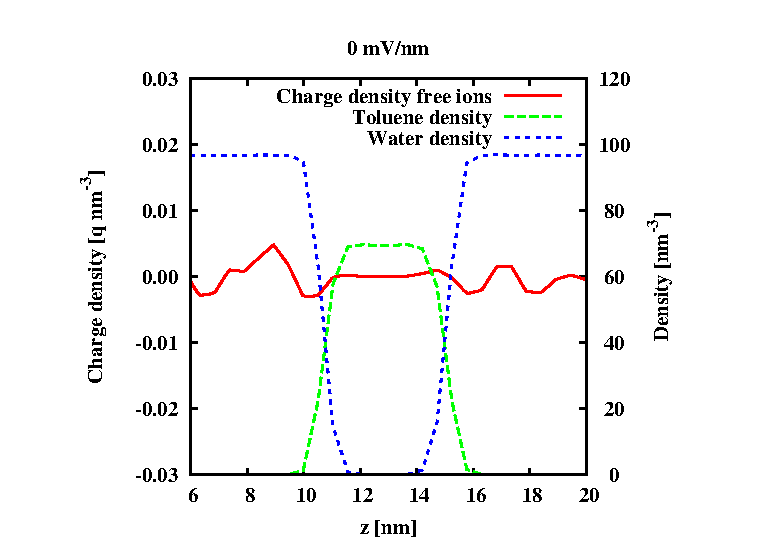
\includegraphics[width=\linewidth]{ST_density_prot_sol_charge_na_cl_0mV.eps}
  \caption{Density distribution at external electric field $0 mV/nm$}
  \label{fig:npt_dens_dist_0mV}
\end{subfigure}%
\begin{subfigure}{.32\textwidth}
  \centering
  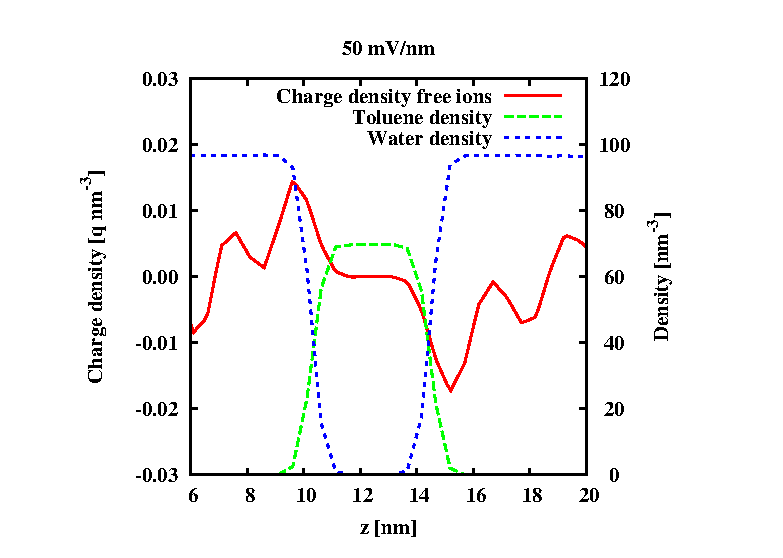
\includegraphics[width=\linewidth]{ST_density_prot_sol_charge_na_cl_50mV.eps}
  \caption{Density distribution at external electric field $50 mV/nm$}
  \label{fig:npt_dens_dist_50mV}
\end{subfigure}
\begin{subfigure}{.32\textwidth}%
  \centering
  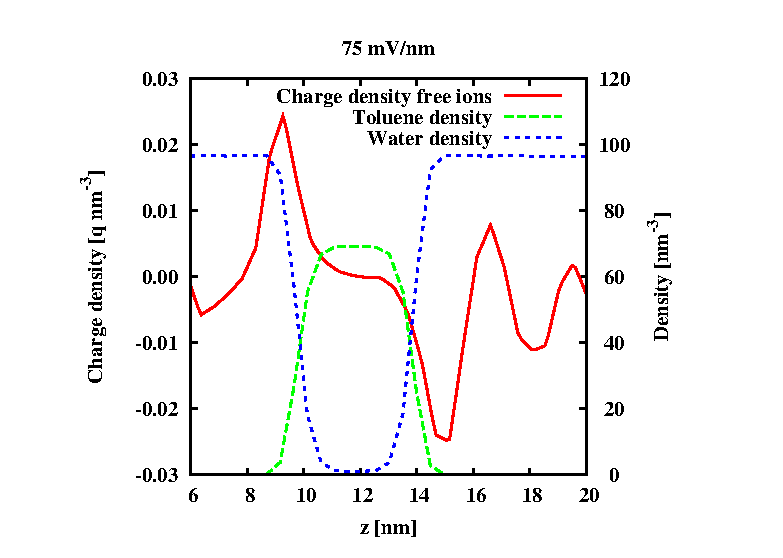
\includegraphics[width=\linewidth]{ST_density_prot_sol_charge_na_cl_75mV_0-1ns.eps}
  \caption{Density distribution at external electric field $75 mV/nm$}
  \label{fig:npt_dens_dist_75mV}
\end{subfigure}
\caption{Density distribution of free ions (red), toluene (green) and water molecules (blue) at different external electric fields in NPT ensemble}.
\label{fig:npt_all_distributions}
\end{figure}
